\section{Results Overview}
\label{sec:comp-results}

The combined results for all tracks are summarized in \Cref{fig:combinedresults},
which shows the total number of benchmarks solved by each solver in various track.
We observe that \cvcnew\ solved the highest combined number of benchmarks,
and \eusolvernew\ solved almost as many.

\begin{figure}
	\centering
	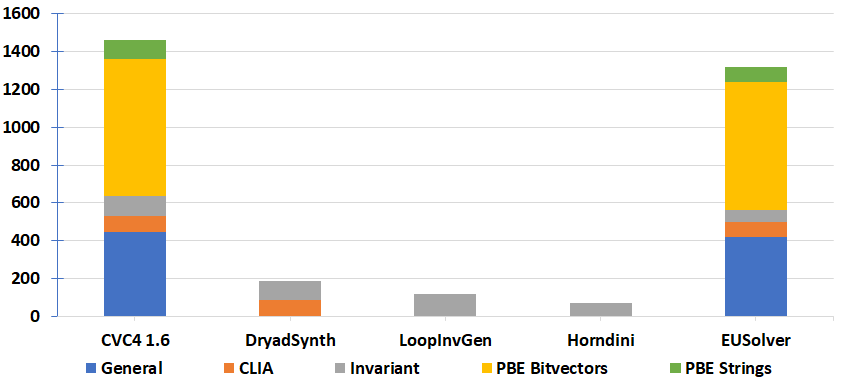
\includegraphics[width=0.95\textwidth]{figures/TotalSolved.png}
	\caption{The overall combined results for each solver on benchmarks from all five tracks.}
	\label{fig:combinedresults}
\end{figure}

The primary criterion for winning a track was the number of benchmarks solved,
but we also analyzed the time to solve and the the size of the generated expressions.
Both were classified using a pseudo-logarithmic scale as follows.
For time to solve, the scale is: $[0,1)$, $[1,3)$, $[3,10)$, $[10,30)$, $[30, 100)$,
$[100,300)$, $[300, 1000)$, $[1000,3600)$, $\geqslant 3600$.
That is, the first ``bucket'' refers to termination in less than one second,
the second to termination in one to three seconds and so on.
We say that a solver solved a certain benchmark \emph{among the fastest}
if the time it took to solve that benchmark is in the same bucket
as that of the solver which solved that benchmark in minimum time.
Similarly, for expression sizes, the pseudo-logarithmic scale we use is:
$[1,10)$, $[10,30)$, $[30,100)$, $[100,300)$, $[300,1000)$, $\geqslant 1000$,
where expression size is the number of nodes in the SyGuS parse-tree.
In some tracks there was a tie or almost a tie in terms of the number of solved benchmarks,
but the differences in the time to solve where significant.
We also report on the number of benchmarks \emph{solved uniquely} by a solver,
\emph{i.e.} the number of benchmarks which no other solver but this particular solver could solve.

\Cref{fig:resultsPerTrack} shows the percentage of benchmarks solved,
the percentage of those among the fastest,
and the percentage of synthesized expressions among the smallest size
for each solver in each track.

\begin{figure}
	\begin{center}
		\begin{minipage}{\textwidth}
			\centering
			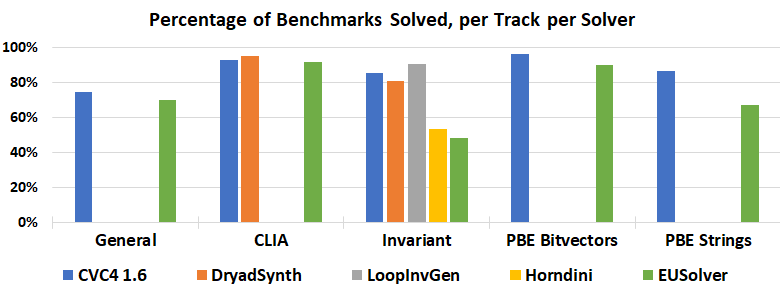
\includegraphics[width=0.95\textwidth]{figures/Solved.png}
		\end{minipage}
		\\[1cm]
		\begin{minipage}{\textwidth}
			\centering
			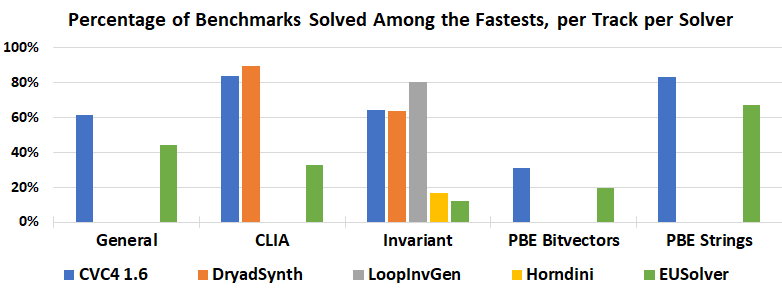
\includegraphics[width=\textwidth]{figures/Fastest.png}
		\end{minipage}
		\\[1cm]
		\begin{minipage}{\textwidth}
			\centering
			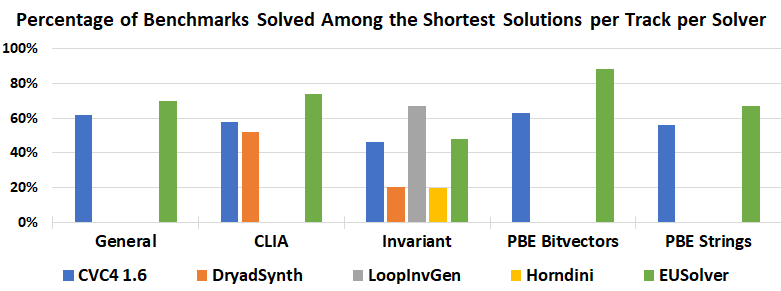
\includegraphics[width=\textwidth]{figures/Smallest.png}
		\end{minipage}
	\end{center}
	\caption{Percentage of benchmarks solved by different solvers across all tracks,
			 the percentage of benchmarks a solver solved among the fastest,
			 and the percentage of benchmarks for which the solver generated an expression among the smallest size.}
	\label{fig:resultsPerTrack}	
\end{figure}

\paragraph{General Track}
In the general track, \cvcnew\ solved more benchmarks than all others ($447$),
and \eusolvernew\ came second, solving $420$ benchmarks.
We note that the new version \cvcnew\ of \cvc, is significantly better than the previous version \cvclast,
which could only solve $395$ benchmarks.
The same order appears in the number of benchmarks solved among the fastest:
\cvcnew\ with 366, \eusolvernew\ with 266, and \cvclast\ with 231.
\verify{In terms of benchmarks solved uniquely by these solvers,
we have that \cvcnew\ solved ??? uniquely and \eusolvernew\ solved ??? uniquely.}

\begin{table}[t]
	\begin{center}
		\scalebox{0.9}{
		\begin{tabular}{lr||rrrrrrrrrrrr|r}
			 &	& \rot{Compiler Optimizations and Bit Vectors}	& \rot{Let and Motion Planning} &	\rot{Invariant Generation with Bounded Ints} &	\rot{Invariant Generation with Unbounded Ints} &	\rot{Multiple Functions}	& \rot{Arrays} &	\rot{Hackers Delight} &	\rot{Integers} &	\rot{Program Repair} &	\rot{ICFP} &	\rot{Cryptographic Circuits} &	\rot{Instruction Selection} & {Total}\\\hline \hline
\multicolumn{2}{l||}{Number of benchmarks}  & 32 & 30 & 28 & 28 & 32 & 31 & 44 & 34 & 18 & 50 & 214 & 28 & 569 \\ \hline			 
\multirow{3}{*}{Solved} & \eusolvernew\ &	16	& 10	& 24	&24 &	18	& 31	& 35 &	33 &	14 &	50& 	152& 	0 & 407 \\
& \cvcnew\ &	15	& 15	& 24	& 24	& 12	& 31 &	44& 	34&	14&	48&	117&	0 & 378 \\
& \euphony\	& 19	&10 &	24 &	24 &	18	& 31	& 44	& 33	& 14	& 50	& 95 &	0 & 362 \\ \hline
\multirow{3}{*}{Fastest} & \eusolvernew\ &	7	&2 	& 12	& 14	& 6	& 5	& 20	& 14 &	13 &	40	& 143 &	0 & 276\\
 & \cvcnew &	11 &	15 &	18	& 19	& 9	& 31 &	44	& 33	& 7& 	19	& 30	& 0 & 236 \\
& \euphony	& 16 &	2	& 8	& 13 &	13 &	4	& 27 &	14 &	9	& 29	& 0& 	0 & 135 \\ \hline
\multirow{3}{*}{Uniquely} & \eusolvernew\ &	0	& 0& 	0	& 0& 	0	& 0& 	0	& 0 &	0	& 0	& 34 &	0 & 34 \\
& \cvcnew &	1	& 5&	0&	0&	1&	0	&0&	1&	1&	0	&0&	0 & 9\\
& \euphony	& 2	& 0	& 0& 	0	& 0& 	0	& 0& 	0	& 0& 	0 &	0	& 0 & 2\\ \hline			
		\end{tabular}}
	\end{center}
	\caption{Solvers performance across all categories of the general track
	\verify{I don't have the per-category results for the General track ... Should we remove this?}}
	\label{tbl:general-categories}
\end{table}

\verify{I don't have the per-category results for the General track ... Should we remove this?}
We partition the benchmarks of the general track according to categories where different categories consists of related benchmarks.
The results per category are given in the Table~\ref{tbl:general-categories}.
We can see that \eusolvernew\ preformed better than others in the categories of program repair, icfp and cryptographic circuits.
The \cvcnew\ solver preformed better than others in the categories of let and motion planning, invariant generation with bounded and unbounded integers,
arrays, integers and hacker's delight. The \euphony\ solver preformed better than others in the categories of
multiple functions, compiler optimizations and bitvectors.
We can also observe that none of the solvers could solve any of the instruction selection benchmarks.

% \begin{figure}
% 	\begin{center}
% 		\begin{minipage}{1\textwidth}
% 			\centering
% 			\includegraphics[scale=0.9,width=1\textwidth]{Figures/GeneralSolved.png}
% 		\end{minipage}
% 		\\
% 		\vspace{2mm}
% 		\begin{minipage}{1\textwidth}
% 			\centering
% 			\includegraphics[scale=0.9,width=1\textwidth]{Figures/GeneralWon.png}
% 		\end{minipage}
% 	\end{center}
% 	\caption{Percentage of benchmarks solved by the different solvers across all categories of the general track, and the percentage of benchmarks a solver solved among the fastest for that benchmark (according to the logarithmic scale).  }	
% \end{figure}	


\paragraph{Conditional Linear Arithmetic Track}
In the CLIA track, \cvcnew\ and \dryd\ had a close competition.
\cvcnew\ solved $85$ out of $88$ benchmarks, \dryd\ solved $84$ benchmarks, and \eusolvernew\ solved $81$ benchmarks.
In terms of the time to solve, \dryd\ solved $79$ benchmarks among the fastest, \cvcnew\ solved $74$,
followed by \eusolvernew\ which solved $29$ among the fastest.
There were $2$ benchmarks that were solved uniquely by \dryd\ and $1$ that was solved uniquely by \cvcnew.

\paragraph{Invariant Generation Track}
In the invariant generation track, the \lig\ solver solved $115$ out of $127$ benchmarks, \cvcnew\ solved $109$,
\dryd\ solved $103$, \horndini\ solved $68$ and \eusolvernew\ solved $61$ benchmarks.
In terms of the time to solve, \lig\ solved $102$ benchmarks among the fastest, followed by \cvcnew\ which solved $82$,
\dryd\ which solved $81$, \horndini\ which solved $21$, and \eusolvernew\ which solved $15$.
There was one benchmark that was solved by a unique solver -- the \texttt{fib_17n.sl} benchmark solved by \lig. 

\paragraph{Programming By Example (Bit Vectors) Track}
In the PBE on the theory of bit vectors track, the \cvcnew\ solver solved $724$ out of $750$ benchmarks
and \eusolvernew\ solved $677$ benchmarks.
In terms of the time to solve, \cvcnew\ solved $508$ benchmarks among the fastest,
and \eusolvernew\ solved $468$.
\verify{what about uniquely solved benchmarks?}

\paragraph{Programming By Example (Strings) Track}
In the PBE track on the theory of strings track, the \cvcnew\ solver solved $102$ out of $118$ benchmarks,
and \eusolvernew\ solved $79$ benchmarks.
In terms of the time to solve, \cvcnew\ solved $98$ benchmarks among the fastest,
and \eusolvernew\ solved $79$.
\verify{what about uniquely solved benchmarks?}